\documentclass[convert]{standalone}

\usepackage{tikz}
\usepackage{pgfplots}
\usepackage{amsmath}
\usetikzlibrary{arrows}

\begin{document}


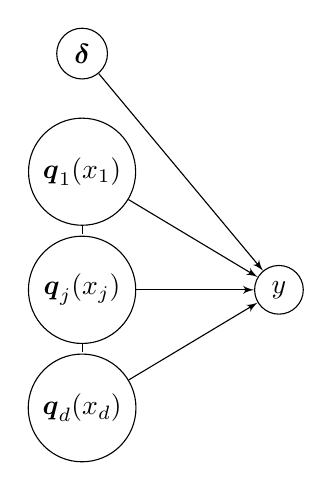
\begin{tikzpicture}
\tikzset{vertex/.style = {shape=circle,draw,minimum size=1.5em}}
\tikzset{edge/.style = {->,> = latex'}}

% vertices

\node[vertex] (delta) at  (2.5,3) {$\boldsymbol{\delta}$};
\node[vertex] (q1) at  (2.5,1.5) {$\boldsymbol{q}_1(x_1)$};
\node[vertex] (qj) at  (2.5,0) {$\boldsymbol{q}_j(x_j)$};
\node[vertex] (qd) at  (2.5,-1.5) {$\boldsymbol{q}_{d}(x_d)$};

\node[vertex] (y) at (5,0) {$y$};

% edges

\draw[edge] (q1) to (y);
\draw[edge] (qj) to (y);
\draw[edge] (qd) to (y);
\draw[edge] (delta) to (y);

% correlation

\draw[dashed] (q1) to (qj);
\draw[dashed] (qj) to (qd);
\end{tikzpicture}


\end{document}